\documentclass[12pt]{article}
\usepackage{natbib}

\usepackage{graphicx}
\usepackage{url}

\begin{document}

\section{Overview}

Image recognition is an important technique in a range of fields, from security and surveillance, to intelligent document scanning. 

Working with the MNIST database of images of handwritten digits (available from \citep{MNIST}), KrisNMel is a function which, when given a set number images to classify, returns the recognised value of those images. This recognised value is determined by comparison with the train data images. 

The KrisNMelpca function uses an improved method (principal component analysis) to identify feature vectors and increase 

Unsupevised methods (ie, methods that don't use training data) are then discussed, particularly in the case of the kmeans algorithm for clustering. It is shown that this method is much less accurate that the supervised method, and areas for improvement are suggested.

\section{Quick links: where to look}

\begin{itemize}
\item{Obtaining and opening the data} 
\item{knn algorithm on intensity and pca method}
\item{knn with different metrics}
\item{Clustering methods}
\end{itemize}

\section{The MNIST data}

%\begin{figure}
%  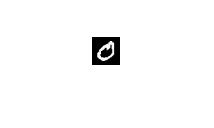
\includegraphics{/home/user/InFoMM/YearOne/WeekTwo/ImageClassificationTask/OpenImages/zero.jpg}
\includegraphics{/home/user/InFoMM/YearOne/WeekTwo/ImageClassificationTask/OpenImages/7.jpg}\includegraphics{/home/user/InFoMM/YearOne/WeekTwo/ImageClassificationTask/OpenImages/9.jpg}
%\end{figure}

The MNIST data stores each image as a 1-d column vector, with each row corresponding to a pixel. images from MNIST are stored vectors of length 784 (corresponding to an image of size 28x28pix). 

The basic principle then is to compare of each image in the test data against the images in the training data set, and find a way to match  (ie. Euclidean distance)   

Matlab will not open binary files. In order to access them therefore, the functions LOAD need to be applied to both the test and training labels.\citep{ahu61}

The appropriate matlab code can be found in the OpenImages folder.

\section{the knn-algorithm}
The knn algorithm is a way of comparing a sample set against a wider data set. For a given a data set (in our case the column vector corresponding to the test image), it identifies the closest values (default metric is Euclidean) from within the training set.

It is important to understand the effect of choosing the appropriate value for \(k\). If the identified neighbours all have the same label, our confidence in the allocated label is greater. However, past a certain point, the chance of identifying incorrect labels increases, as matched images become further away from the test image.

Fig \ref{errork} illustrates effect of error of increasing \(k\) in the case ***.

\section{Applying to the Intensity Matrix}

Initially, the knn algorithm was applied to the whole vector length, for test samples of size 1,000. The error in this case was roughly 3%.

However, a significant issue with this method was the length of time taken for the algorithm to run. A simple way to reduce this is to reduce the number of training images against which the test images are matched. Fig \ref{errortrain} illustrates the effect of increasing the number of training images to compare against. In this case, the error is largely unchanged whether we include 40,000 or the full 60,000.

However, by manipulating the data from the test images, we are able to reduce the time taken to run even further, without reducing the number of trianing images to compare against. This is because lots of information contained in the vector is irrelevant to its final class (eg lighting conditions, discrepancies in the orientation of the shape).

\section{PCA}

Principal component analysis is a way of identifying key features within a matrix. The process transforms the data to a coordinate system where the greatest variation lies on on the first co-ordinate (\emph{first principal components}). These components are also referred to as \emph{feature vectors} as the describe key features of the data. For a comprehensive review of the method, see \citep{PCA}.

We can then disregard all but the first \emph{n} feature vectors, which will increase the speed of the algorithm whilst maintaining the accuracy. 

Another alteration is to discard the first few feature vectors as well, as these will correspond to generic features of the whole data set (eg. lighting conditions). Within the code, this can be done by specifying \emph{d} as the number of early vectors to neglect. Note that any gains from doing this will be lost if \emph{d} is too large. Generally a value of 2 or 3 will achieve an increase in acccuracy and a decrease in cost. 

Fig \ref{errorfeat} illustrates the effect of increasing the number of feature vector on decreasing the error. In this case, 20 feature vectors are enough to achieve a high degree of accuracy, whilst significantly reducing the cost. 

\section{Changing the metric}

Another aspect to consider is how distance between images should be measured. This is because Euclidean distance is not always best fitted to identify when images are very similar but have been altered through, for example have been rotated or translated.

A number of different metrics were considered which included; the spearman norm, \emph{'spearman'}, which considers the rank Spearman's coefficient between vectors, the cosine norm, \emph{'cosine'}, which considers one minus the interior angle between points, and the correlation norm, \emph{'correlation'}, which considers one minus the sample correlation between points. In all three cases, both the error and time taken to run decreased, most notably with the correlation norm.

These changes are indicated within the 'Intensityerror.m' file in Code.

\section{Results - Computation Speed and Error}

\section{Unsupervised case}

The knn algorithm relies on a large sample of training data with which to compare images. Not only is this costly, it is not always possible to build such a set, and hence it is interesting to consider how unsupervised learning

The file 'kmeanserror.m' looks at applying the kmeans algorithm to a sample of test data to sort it. This algorithm works by intialising a set of 'cluster means', assigning each data point to its nearest cluster mean, and then recursively recalculating the mean of all the elements in the cluster and reassigning elements to their new closest mean. Note that wince we know the number of classes must correspond to the number of digits, we do not have any difficulty using a cluster method which requires knowing the number of clusters in advance. 

It was found that the method had quite high error, and different digits were frequently sorted into the same cluster (see fig. \ref{cluster}). In order to improve the accuracy of the method, the vectors need to be treated such that the differences between those of different classes are emphasised and those within classes are downplayed. Methods similar to those outlined above for the training data approach may be useful in pursuing this further.

\begin{figure}
  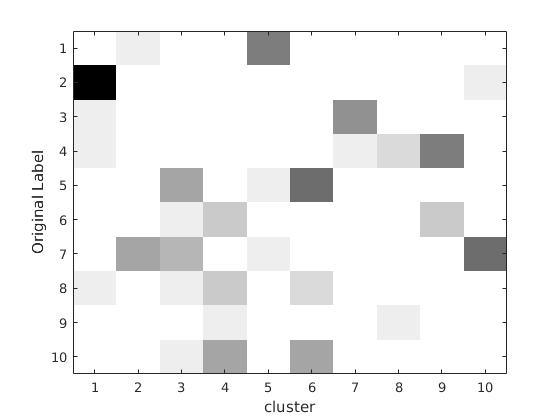
\includegraphics[width=\linewidth]{/home/user/InFoMM/YearOne/WeekTwo/ImageClassificationTask/clustering/kmeanscluster5000.jpg}
  \caption{The clusters generated by kmeans for 5000 images. Here, most of the clusters only have one or two digits represented, but some have as many as five, suggesting kmeans needs refining to make it more accurate.}
  \label{fig:cluster}
\end{figure}



\bibliographystyle{plain}
\bibliography{bibtry}

\end{document}



http://ufldl.stanford.edu/wiki/index.php/Using_the_MNIST_Dataset
